\documentclass[aspectratio=169]{beamer}

\usepackage[utf8]{inputenc}
\usepackage{array}
\usepackage{booktabs}
\usepackage{bold-extra}
\usepackage{graphics}
\usepackage{hyperref}
\hypersetup{%
  colorlinks=true,
  linkcolor=blue,
  filecolor=blue,
  urlcolor=cyan,
}
\usepackage{listings}
\usepackage{multicol}
\usepackage[absolute,overlay]{textpos}
\usepackage{setspace}
\usepackage{verbatim}
\usepackage{fancyvrb} % for verbatim centering
\usepackage{tikz}

\usetheme{Warsaw}
\usecolortheme{beaver}
\definecolor{clOrange}{HTML}{E76600}
\definecolor{clAlmostWhite}{HTML}{FEFFD9}
\definecolor{clGreen}{HTML}{007F00}
\definecolor{clFlag}{HTML}{D33682}
\definecolor{clFlagOpt}{HTML}{CB4B16}
\definecolor{clRedFlag}{HTML}{DC322F}
\definecolor{clViolet}{HTML}{4c0070}

\definecolor{clCodeBlue}{rgb}{0.0, 0.18, 0.38}
\definecolor{clCodeGreen}{rgb}{0.0, 0.27, 0.15}
\definecolor{clCodeRed}{rgb}{0.63, 0.0, 0.0}


\setbeamertemplate{navigation symbols}{}
\setbeamercolor{title}{fg=black}
\setbeamercolor{author}{fg=clAlmostWhite}
\setbeamercolor{date}{fg=clAlmostWhite}
\setbeamerfont{author}{size=\huge}
\setbeamerfont{date}{size=\Large}

\newcommand{\greenemph}[1]{\textit{\textcolor{clGreen}{#1}}}
\newcommand{\cpp}[1]{\texttt{\textbf{\textcolor{clCodeBlue}{#1}}}}

\newcommand\fontV{\fontsize{5}{5}\selectfont}

\lstset{
  language=C++,
  basicstyle=\ttfamily,
  keywordstyle=\color{clCodeBlue}\ttfamily,
  stringstyle=\color{clCodeGreen}\ttfamily,
  commentstyle=\color{clCodeRed}\ttfamily,
  morecomment=[l][\color{magenta}]{\#}
}

\title[Friends\#10 :: \cpp{constexpr}]{\cpp{constexpr}\\
or\\
the evolution of const-ness in recent years
}
\author{Adam Graliński}
\date[FFFE\_21]{\textbf{C++ {\color{red}F}{\color{blue}F}{\color{green}F}{\color{yellow}E}, October 2021}}

\begin{document}

{\usebackgroundtemplate{%
 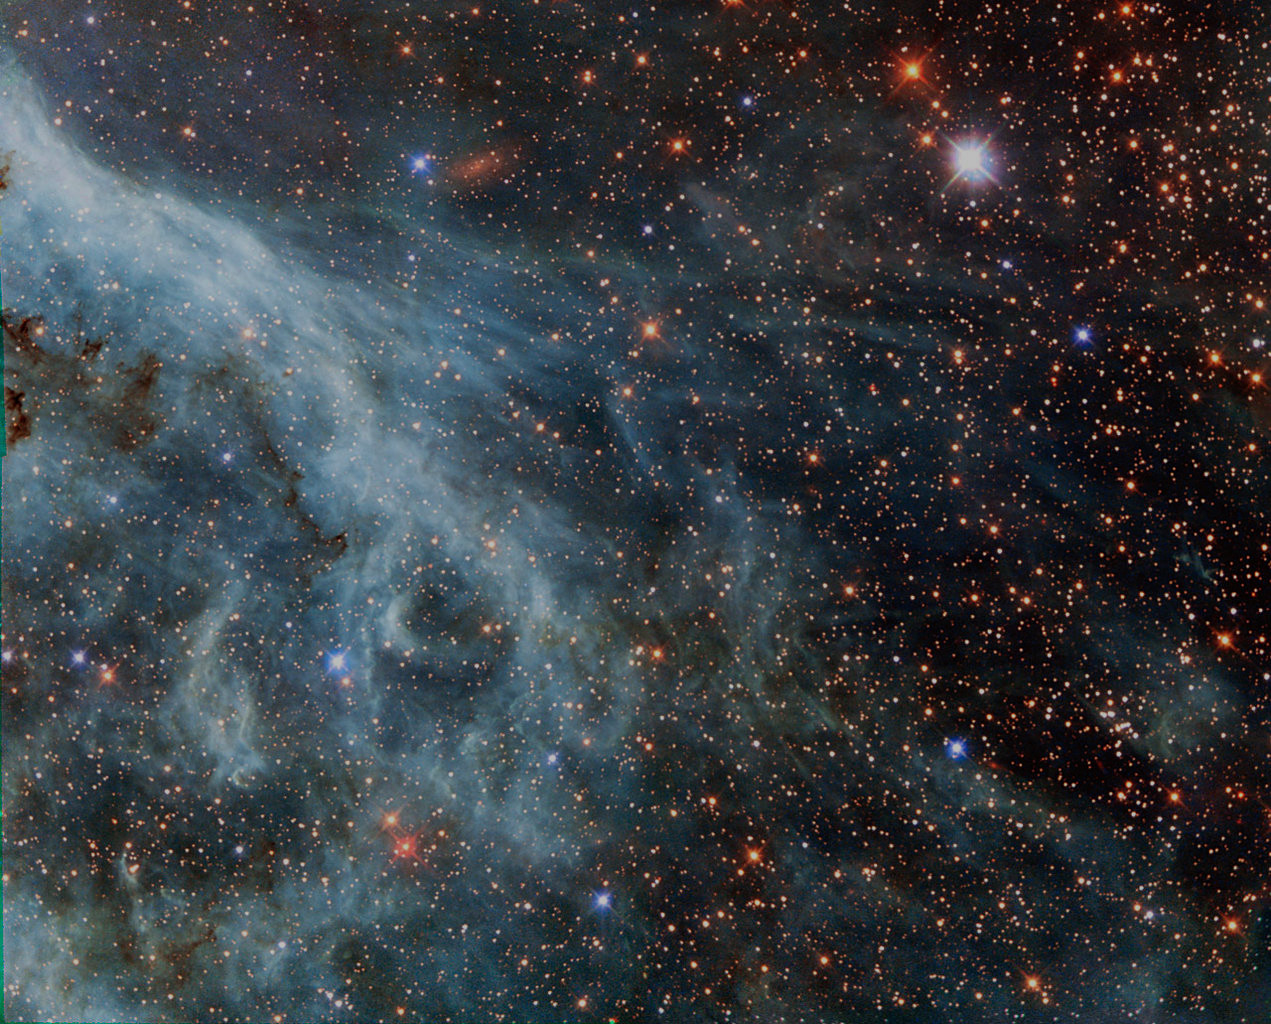
\includegraphics[width=\paperwidth,height=\paperheight]{../common/bg_galaxy.jpg}}
\begin{frame}
\titlepage{}
\end{frame}
}

\begin{frame}
\frametitle{A quick reminder}
You are welcome to:
\begin{itemize}
  \item{interrupt me}
  \item{ask questions immediately :-)}
\end{itemize}
\end{frame}

\begin{frame}[fragile]
\frametitle{cv-type qualifiers}
\href{https://en.cppreference.com/w/cpp/language/cv}{en.cppreference.com/w/cpp/language/cv}
\vspace{6pt}
  \begin{itemize}
    \item<2->{\cpp{const}}
    \begin{itemize}
      \item{defines that the type is \textit{constant} \hspace{2em} \uncover<5->{\textcolor{clGreen}{$\leftarrow{}$ (non-mutable)}}}
      \begin{lstlisting}
        const auto x = 13;
      \end{lstlisting}
    \end{itemize}

    \vspace{3pt}
    \item<3->{\cpp{(no qualifier)}}
    \begin{itemize}
      \item{the type is* a standard \textit{variable} \hspace{2.4em} \uncover<5->{\textcolor{clOrange}{$\leftarrow{}$ (mutable)}}}
      \begin{lstlisting}
        auto x = 13;
      \end{lstlisting}
    \end{itemize}

    \vspace{3pt}
    \item<4->{\cpp{volatile}}
    \begin{itemize}
      \item{the type is \textit{volatile} \hspace{7.8em} \uncover<5->{\textcolor{clRedFlag}{$\leftarrow{}$ (extremely mutable)}}}
      \begin{lstlisting}
        volatile auto x = 13;
      \end{lstlisting}
    \end{itemize}
  \end{itemize}
\end{frame}

\begin{frame}
\frametitle{cv-type qualifiers demo}
  \begin{columns}
    \begin{column}{0.45\textwidth}
      {\fontsize{8}{8} \lstinputlisting{code/01_cvspec.cpp}}
    \end{column}
    \begin{column}{0.55\textwidth}
      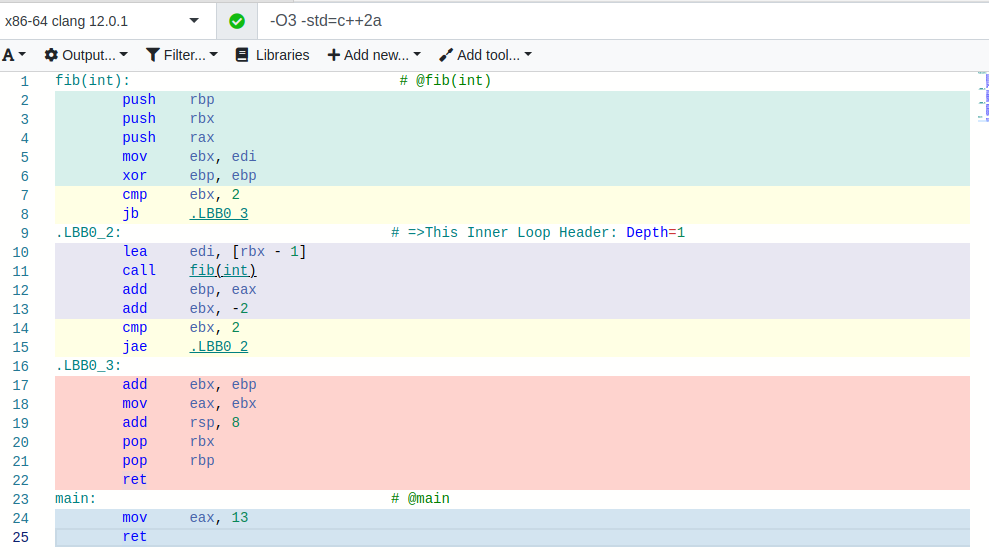
\includegraphics[width=\textwidth]{pics/01_cvspec_assembly}
    \end{column}
  \end{columns}
\end{frame}


\begin{frame}
\frametitle{\cpp{constexpr} --- C++11}
\href{https://en.cppreference.com/w/cpp/language/constexpr}{en.cppreference.com/w/cpp/language/constexpr}\\ \vspace{12pt}
{\footnotesize
\cpp{constexpr} --- specifies that the value of a variable or function can appear in constant expressions\\ \vspace{6pt}
A \textbf{constexpr function} must satisfy the following requirements:
  \begin{itemize}
    \item{it must not be virtual \textcolor{clGreen}{(until C++20)}}
    \item{its return type (if any) must be a LiteralType}
    \item{each of its parameters (if any) must be a LiteralType}
    \item{for constructor (...), the class must have no virtual base classes}
  \end{itemize}
}
\end{frame}


\begin{frame}
\frametitle{switching to a constexpr...}
  \begin{columns}
    \begin{column}{0.45\textwidth}
      {\fontsize{8}{8} \lstinputlisting{code/02_constexpr.cpp}}
    \end{column}
    \begin{column}{0.55\textwidth}
      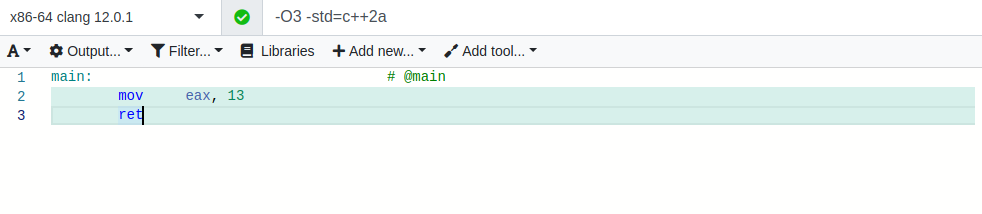
\includegraphics[width=\textwidth]{pics/02_constexpr_assembly}
    \end{column}
  \end{columns}
\end{frame}

\begin{frame}
\frametitle{\cpp{constexpr} or \cpp{consteval}?}
\href{https://godbolt.org/z/4cv71W}{godbolt.org/z/4cv71W}\\
\vspace{12pt}
  \begin{columns}<2->
    \begin{column}{0.45\textwidth}
      {\fontsize{8}{8} \lstinputlisting{code/03_consteval.cpp}}
    \end{column}
    \begin{column}{0.55\textwidth}
      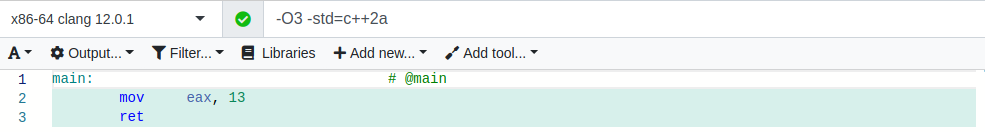
\includegraphics[width=\textwidth]{pics/03_consteval_assembly}
    \end{column}
  \end{columns}
\end{frame}

\begin{frame}
\frametitle{Caveat: exceptions}
the function body must not contain: a try-block\textsuperscript{\textcolor{clGreen}{* relaxed for C++20}} \\
\begin{columns}
  \begin{column}{0.45\textwidth}
    {\fontsize{8}{8} \lstinputlisting{code/04_dont_use_exceptions.cpp}}
  \end{column}
  \begin{column}{0.5\textwidth}
    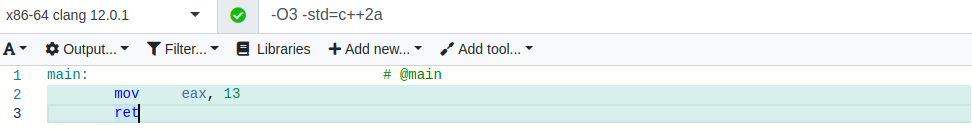
\includegraphics[width=\textwidth]{pics/04_success_when_not_thrown.png}\\
    \vspace{36pt}
    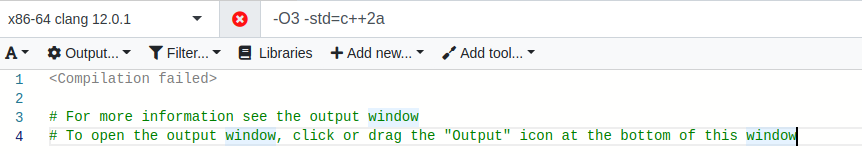
\includegraphics[width=\textwidth]{pics/04_failed_when_thrown.png}\\
  \end{column}
\end{columns}
\end{frame}

\begin{frame}
\frametitle{Caveat: stepping outside \texttt{LiteralType}s}
the function's signature...
\begin{itemize}
  \item{...return type must be a \texttt{LiteralType}}
  \item{...each of its parameters must be a \texttt{LiteralType}}
\end{itemize}
\vspace{12pt}
\begin{columns}
  \begin{column}{0.45\textwidth}
    {\fontsize{7}{7} \lstinputlisting{code/05_not_literal_types.cpp}}
  \end{column}
  \begin{column}{0.5\textwidth}
    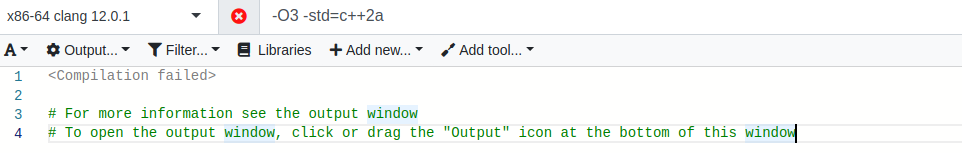
\includegraphics[width=\textwidth]{pics/05_not_a_LiteralType.png}\\
  \end{column}
\end{columns}
\texttt{error: constexpr variable cannot have non-literal type `const Point'}
\end{frame}


\begin{frame}
\frametitle{Caveat: cryptic arcane stuff from the ,,do not open'' bag}
the function body must not contain:
\begin{itemize}
  \item{\cpp{goto} statements}
  \item{labels other than \cpp{case} and \cpp{default}}
  \item{asm blocks}
\end{itemize}
\vspace{24pt}
But you're already \textbf{not using them}.
\end{frame}

\begin{frame}
\frametitle{Taste of the future: \cpp{constexpr std::string}, \cpp{std::array}, \cpp{std::vector}}
\begin{center}
  \texttt{C++ Weekly \#269}: \href{https://www.youtube.com/watch?v=cuFILbHp-RA}{youtube.com/watch?v=cuFILbHp-RA}\\
  
\includegraphics[width=0.35\textwidth]{pics/cppweekly269.png}
\end{center}

\begin{itemize}
  \item{Sort your \cpp{std::vector} of \cpp{std::string}s at compile time!}
  \item{\cpp{std::accumulate()} your \cpp{std::vector} of doubles at compile time!}
  \item{\textcolor{clGreen}{-std=C++20} and not yet implemented by your compiler vendor!}
  \begin{itemize}
    \item{...but some fastring insider previev of \texttt{MSVC} has/had it!}
    \item{...while both \texttt{clang++} \& \texttt{g++} support constexpr constructors now}
  \end{itemize}
\end{itemize}
\end{frame}

\begin{frame}
\frametitle{Taste of the future: \cpp{consteval if} (\textcolor{clGreen}{\texttt{C++23}})}
  \href{https://en.cppreference.com/w/cpp/language/if\#Consteval\_if}{en.cppreference.com/w/cpp/language/if\#Consteval\_if}
\end{frame}

\begin{frame}
\frametitle{Key takeaways}
{\centering
\begin{itemize}
  \item{Make your constant expressions \cpp{const} or \cpp{constexpr}}
  \item{Make your functions \cpp{consteval} or \cpp{constexpr} where possible}
  \item{No downsides!}
  \item{Be aware of the ,,slow march of progress'' across C++ standards}
  \item{Be aware of the lag in compiler implementations for C++20 features}
\end{itemize}

\vspace{2ex}
\begin{center}{\Large Thank you!}\end{center}
}
\end{frame}

\end{document}
